% !TeX root = ../main.tex
% Add the above to each chapter to make compiling the PDF easier in some editors.

\chapter{Approach}\label{chapter:approach}

\section{Skip List}

A skip list is a probabilistic data structure that allows fast search, insertion, and deletion. It is an alternative to balanced trees, such as AVL trees or red-black trees~\parencite{pugh1990skip, pugh1990skip2}. The key idea of a skip list is to use multiple layers of sorted linked lists to maintain elements, where each layer is an "express lane" for faster traversal.

\begin{figure}[h]
    \centering
    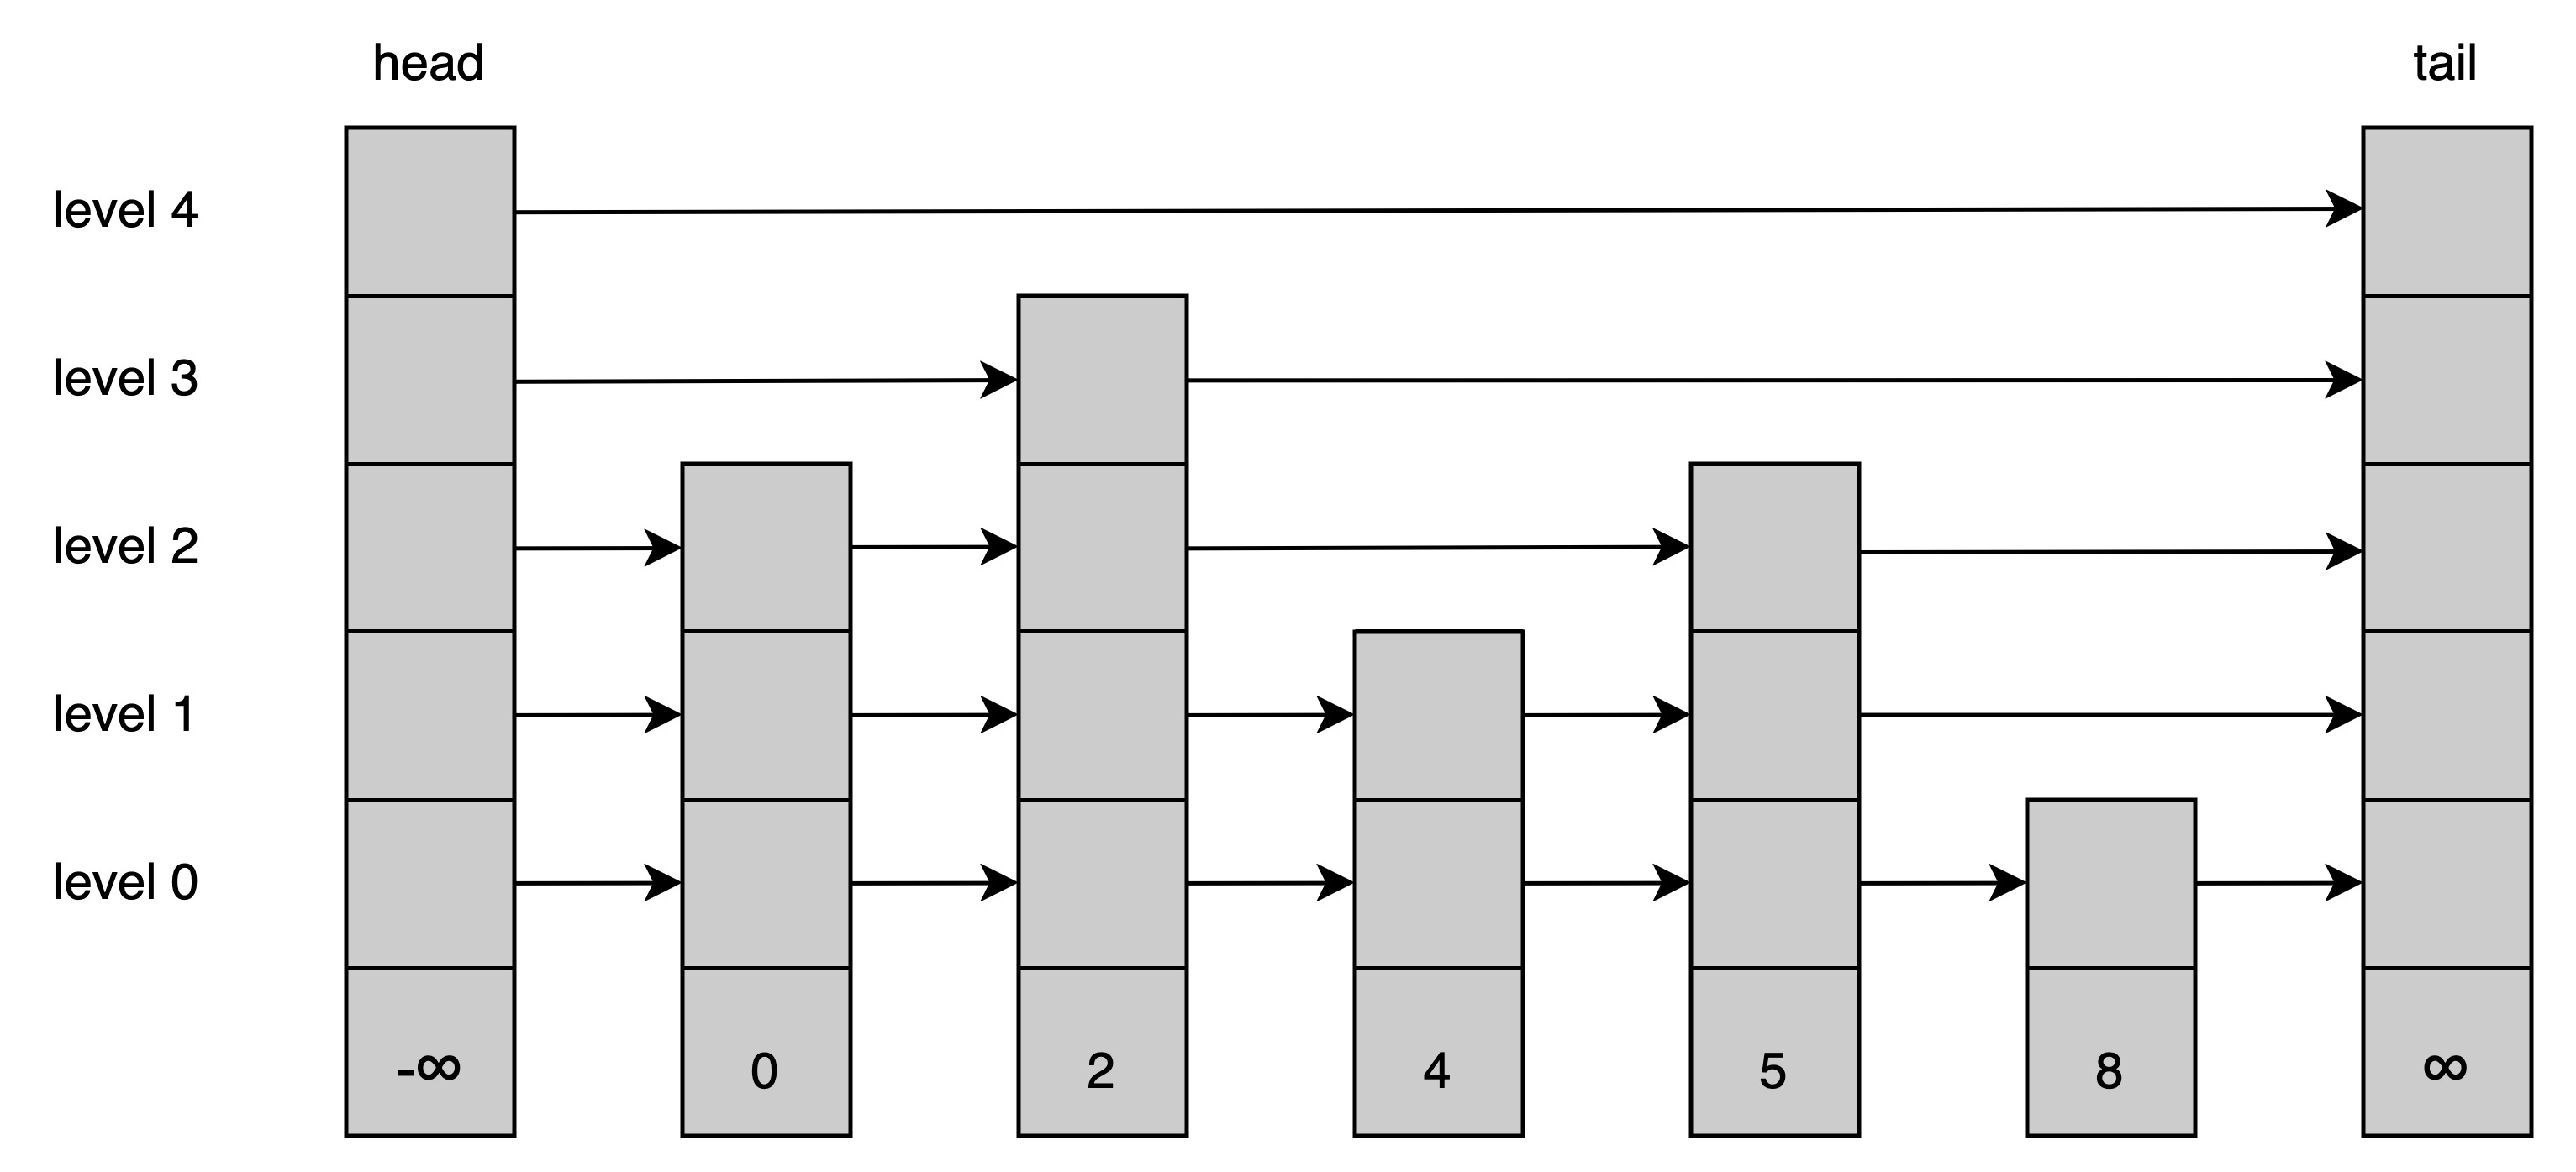
\includegraphics[width=0.8\textwidth]{./figures/skiplist.jpg}
    \caption{Skip List: this example has five levels of sorted linked lists. \\
    Each node has an unique key, and the head and tail have $-\infty$ and $+\infty$ keys.}
    \label{fig:skiplist}
\end{figure}

\subsection*{How it work}

\textbf{Layers:} A skip list consists of multiple layers. The bottom-most layer is a regular sorted linked list. Each higher layer acts as an "express lane" to speed up access by skipping over multiple elements from the layer below.

\textbf{Probabilistic Balancing:} When a new element is inserted, a node with a random height is generated. This random generation ensures that the list structure remains balanced. Consequently, skip list insertion and deletion algorithms are much simpler and faster than equivalent algorithms for balanced trees.

\textbf{Search Operation:} To search for an element, the search starts at the top-most layer and moves horizontally until it finds an element greater than or equal to the target element. If it finds an element greater than the target, it drops to the next lower layer and continues the search. This process repeats until the element is found or the search reaches the bottom-most layer without finding the target.

\textbf{Insertion and Deletion:} Inserting an element involves placing it in the appropriate position in the bottom-most layer and then possibly promoting it to higher layers based on the coin flips. Deleting an element involves removing it from all layers in which it appears.

\begin{figure}[h]
    \centering
    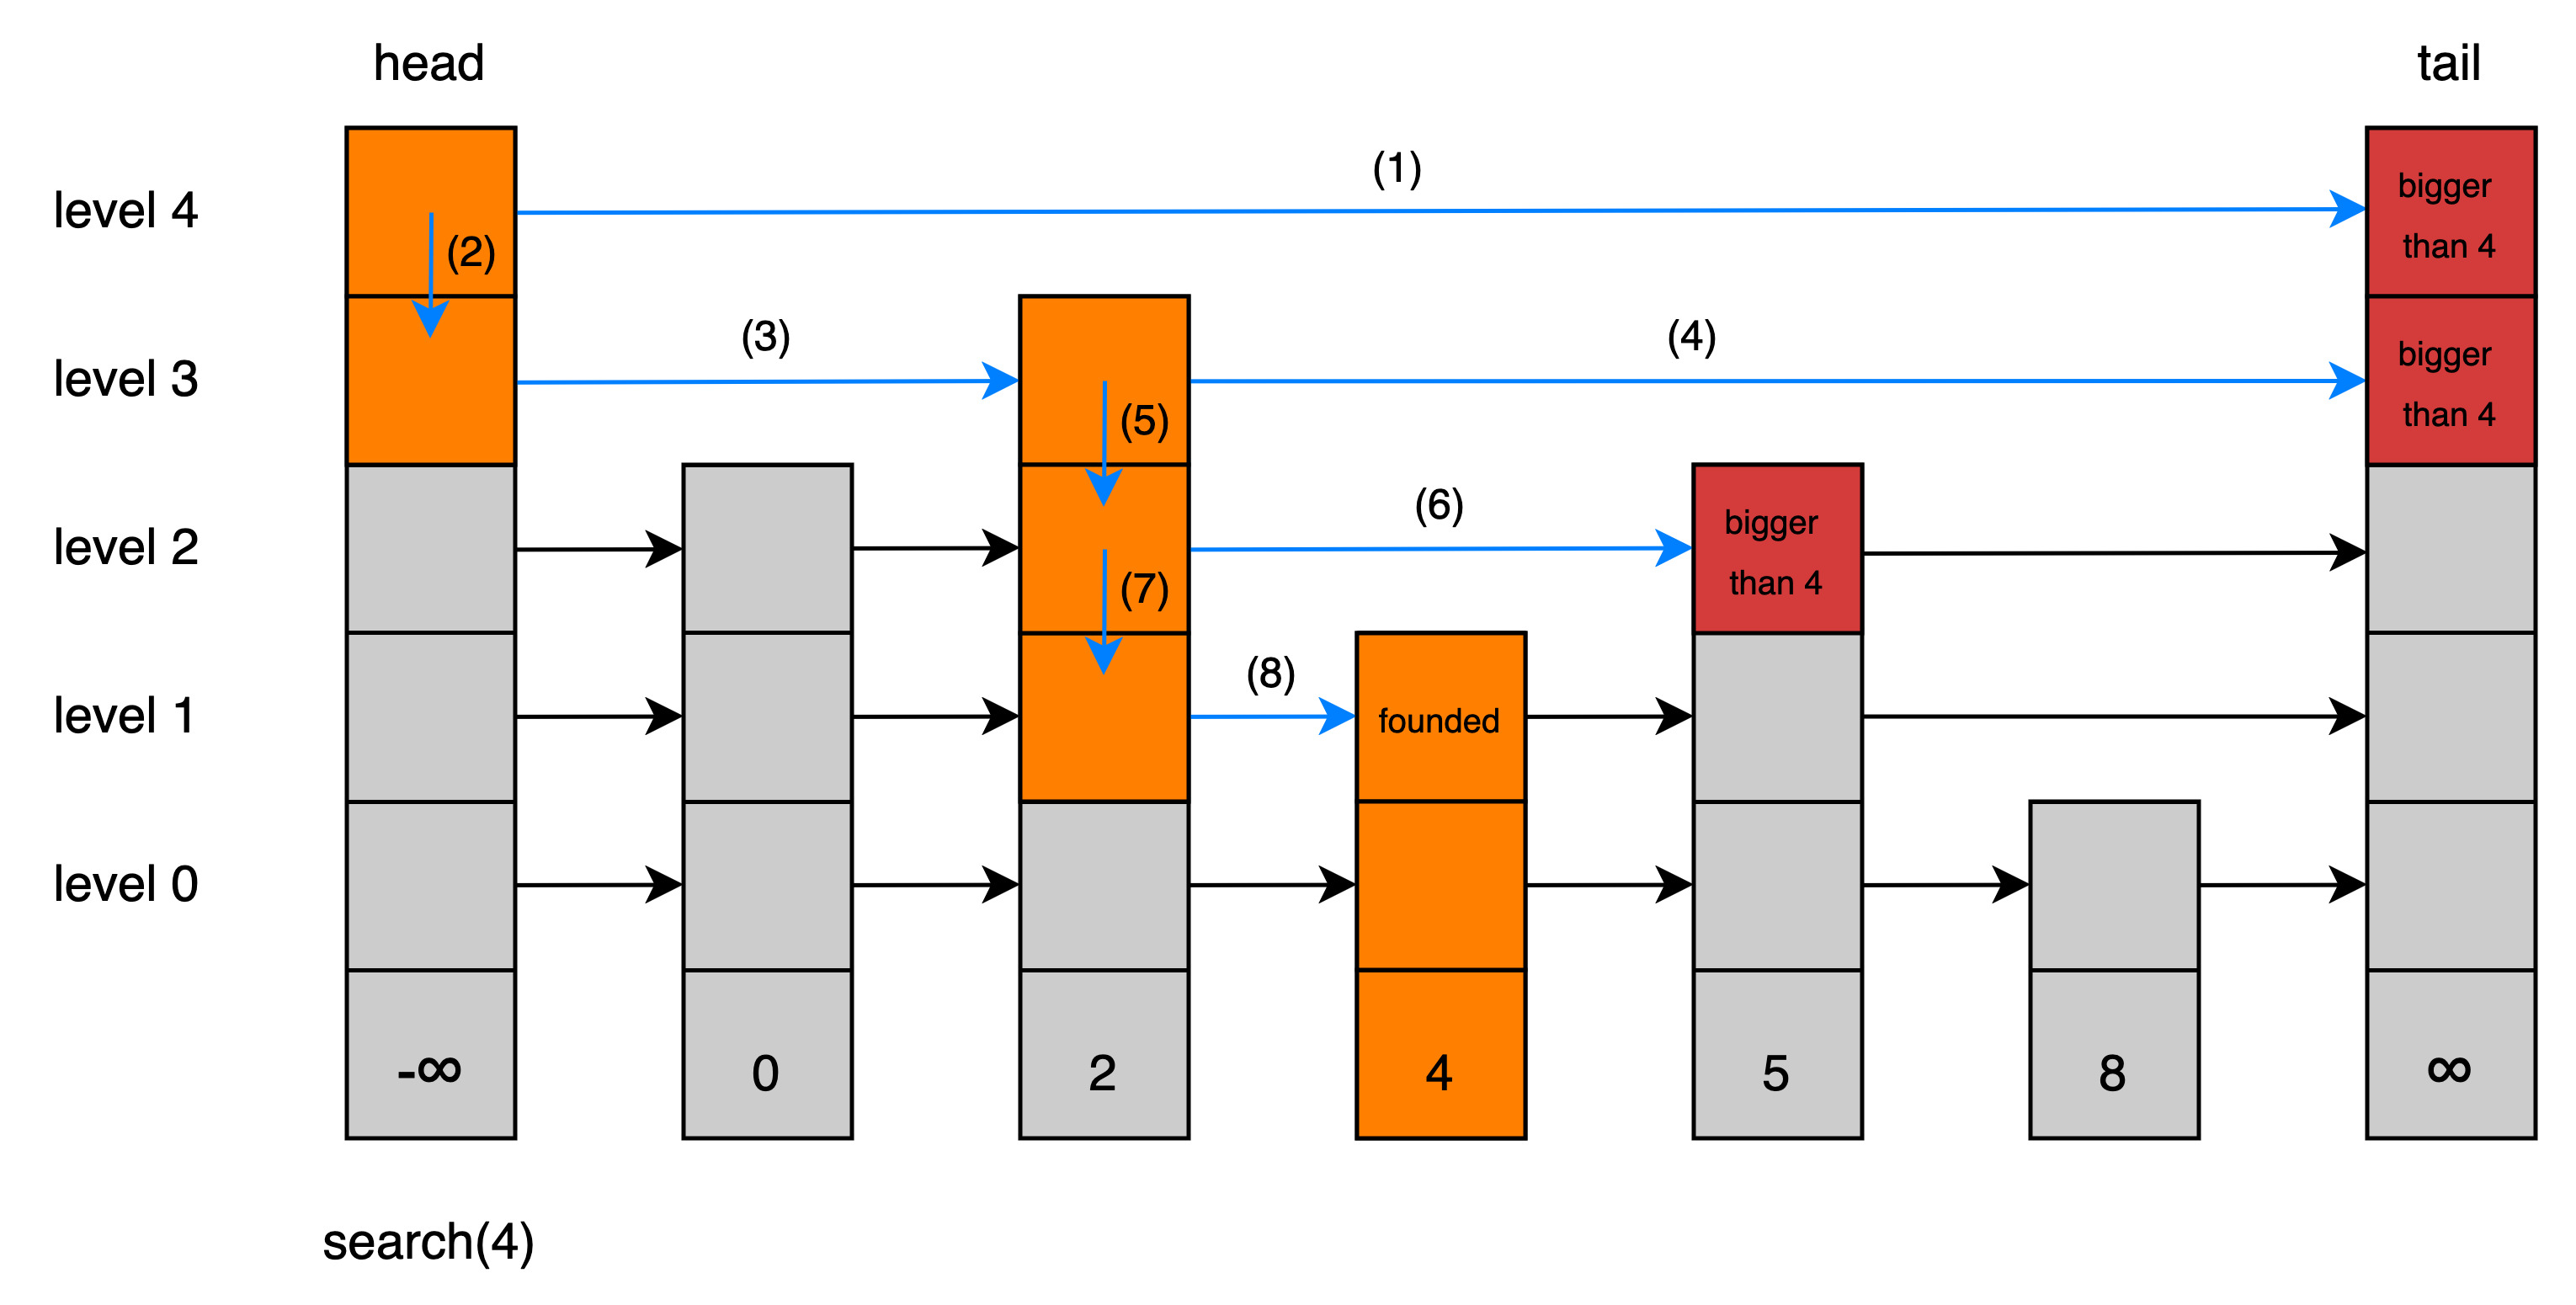
\includegraphics[width=0.8\textwidth]{./figures/skiplistsearch.jpg}
    \caption{Skip List: In this example, the list searches for a node with value 4. It starts on the head node on the highest level, tries to move horizontally until it reaches a greater value than 4, and then goes down a level and repeats. The number noted on the arrows implies the order of the traversal.}
    \label{fig:skiplistsearch}
\end{figure}

Despite their theoretically poor worst-case performance, skip lists rarely exhibit worst-case behavior, making them efficient in most scenarios. For instance, in a dictionary with over 250 elements, the likelihood of a search taking more than three times the expected duration is less than one in a million~\parencite{pugh1990skip2}. Skip lists are ideal for implementing range locks, offering a balanced structure that improves concurrency.


\begin{table}[h!]
    \centering
    \begin{tabular}{|c|c|c|c|}
        \hline
        \textbf{Operation} & \textbf{Best Case} & \textbf{Average Case} & \textbf{Worst Case} \\ \hline
 Search, Insert, Delete & $O(1)$ & $O(\log n)$ & $O(n)$ \\ \hline
    \end{tabular}
    \caption{Time complexities of skip list operations. They have the same complexities}
    \label{table:skiplisttimecomplexity}
\end{table}

\newpage

\section{Concurrent Range Lock}